\chapter{Getting Started}

\section{Documentation Conventions}

Items to be selected from a menu are displayed in \menustyle{monospace font}.

Multilevel menu paths are separated by a / character. For example, \menustyle{Attenuation / 1x} means to open the
\menustyle{Attenuation} submenu and select the \menustyle{1x} item.

If there are multiple options for a menu or configuration option, they are displayed in square brackets and separated
by a | character. For example, \menustyle{Move waveform to / Waveform Group [1|2]} means to select either
\menustyle{Waveform Group 1} or \menustyle{Waveform Group 2} from the \menustyle{Move waveform to}
menu.

This project is under active development and is not anywhere near feature complete! As a result, this document is
likely to refer to active bug or feature request tickets on the GitHub issue trackers. Issues are referenced as
repository:ticket, for example scopehal-apps:3.

\section{Host System Requirements}

The majority of development is performed on Linux operating systems (primarily Debian and Arch), although experimental
Windows support is available. glscopeclient uses gtkmm as the UI toolkit. Current development mostly uses 3.24 but any
recent 3.x version should work.

Any 64-bit Intel or AMD processor should be able to run glscopeclient. If AVX2 and/or AVX512F support is present
glscopeclient will use special optimized versions of some signal processing functions, however neither instruction set
is required. Compiling in 32-bit mode is not supported due to the significant RAM requirements.

A mouse with scroll wheel, or touchpad with scroll gesture support, is mandatory to enable full use of the UI. We may
explore alternative input methods for some UI elements in the future.

OpenGL 4.2 or later is required, as well as several extensions:
\begin{itemize}
\item GL\_ARB\_arrays\_of\_arrays (or OpenGL 4.3)
\item GL\_ARB\_compute\_shader (or OpenGL 4.3)
\item GL\_ARB\_shader\_storage\_buffer\_object (or OpenGL 4.3)
\item GL\_EXT\_blend\_equation\_separate
\end{itemize}

The corresponding minimum hardware requirement is an AMD Radeon HD 5000, NVIDIA GeForce GTX 6xx series discrete GPU, or
Intel Skylake or newer integrated GPU, plus suitably up-to-date drivers. On Linux with recent Mesa, Intel integrated
GPUs as old as Ivy Bridge may be used.

TODO: what AMD integrated/ARM GPUs started supporting GL 4.2?

To check for necessary graphics card support on Linux:
\begin{lstlisting}[language=sh]
glxinfo | grep GL\_ARB\_arrays\_of\_arrays
glxinfo | grep GL\_ARB\_compute\_shader
glxinfo | grep GL\_ARB\_shader\_storage\_buffer\_object
glxinfo | grep GL\_EXT\_blend\_equation\_separate
glxinfo | grep "OpenGL version string"
\end{lstlisting}

If OpenCL 1.2 or higher is present, some filters may make use of GPU acceleration. As of this writing the first
detected GPU is automatically used; there may be a way to select specific devices in the future.

The minimum RAM requirement to actually launch glscopeclient is relatively small (TODO: do some testing) however
history mode and deep captures can easily consume many GB of RAM very rapidly. We suggest 8GB as a reasonable minimum,
with 32 or more encouraged for deep history.

\section{Instrument Support}

glscopeclient uses the libscopehal library to communicate with oscilloscopes, so any libscopehal-compatible hardware
should work with glscopeclient. See the \hyperref[sec:drivers]{Oscilloscope Drivers} section for more details on which
hardware is supported and how to configure specific drivers.

\section{Compilation}

glscopeclient can be compiled on both Linux and Windows, but the specific steps that have to be taken differ quite a
lot between these the two.

\subsection{Linux}
\begin{enumerate}

\item Install dependencies.

On Debian/Ubuntu:

\begin{lstlisting}[language=sh]
sudo apt install build-essential cmake pkg-config libglm-dev \
	libgtkmm-3.0-dev libsigc++-2.0-dev libyaml-cpp-dev \
	liblxi-dev texlive texlive-fonts-extra libglew-dev \
	catch2 libclfft-dev
\end{lstlisting}

On Fedora:

\begin{lstlisting}[language=sh]
sudo dnf install gtkmm30-devel cmake pkg-config glm-devel \
	texlive libyaml-devel yaml-cpp-devel glew-devel \
	catch-devel
\end{lstlisting}

If you are using an older stable release (such as Debian Buster), you may need to install catch2 from source
(https://github.com/catchorg/Catch2). Alternatively, you may pass -DBUILD\_TESTING=OFF to CMake to disable unit testing.

\item Install FFTS library:

\begin{lstlisting}[language=sh]
git clone https://github.com/anthonix/ffts.git
cd ffts
mkdir build
cd build
cmake .. -DENABLE_SHARED=ON
make -j4
sudo make install
\end{lstlisting}

\item Build scopehal and scopehal-apps:

\begin{lstlisting}[language=sh]
git clone https://github.com/azonenberg/scopehal-apps.git --recurse-submodules
cd scopehal-apps
mkdir build
cd build
cmake ../ -DCMAKE_BUILD_TYPE=RELEASE -DCMAKE_INSTALL_PREFIX=/usr
make -j4
\end{lstlisting}

\item Install scopehal and scopehal-apps:

\begin{lstlisting}[language=sh]
make install
\end{lstlisting}

\end{enumerate}

\subsection{Windows}

On Windows, we make use of the MSYS2 development environment, which gives us access to the MingGW-w64 toolchain.
Since this toolchain allows glscopeclient to be compiled as a native Windows application, the project might be run
outside of MSYS2.

Note that glscopeclient is available as a package in MSYS2 repositories.
Therefore, it can be installed through the package manager, without building it from sources:

\begin{lstlisting}[language=sh]
pacman -Sy
pacman -S mingw-w64-x86_64-scopehal-apps
\end{lstlisting}

See also \href{https://packages.msys2.org/group/mingw-w64-x86_64-eda}{\lstinline{mingw-w64-x86_64-eda}}.

\begin{enumerate}

\item Download and install MSYS2. You can download it from \href{https://www.msys2.org/}{msys2.org} or \href{https://github.com/msys2/msys2-installer/releases}{github.com/msys2/msys2-installer/releases}\\
It is of utmost importance that \textbf{all} steps outlined on the website are followed precisely, even if they might
seem unnecessary.
This will avoid lots of hard to diagnose problems later on in the build.\\

All following steps are to be done in a MinGW64 shell (\textbf{not} in a MSYS, MINGW32, CLANG64, CLANG32 or UCRT64 shell,
which also get installed by the MSYS2 installer).

\item Install git and the toolchain:

\begin{lstlisting}[language=sh]
pacman -S git mingw-w64-x86_64-toolchain
\end{lstlisting}

\item Execute makepkg-mingw in subdir MSYS2:

\begin{lstlisting}[language=sh]
cd msys2
MINGW_ARCH=mingw64 makepkg-mingw --noconfirm --noprogressbar -sCLf
\end{lstlisting}

The unit tests will not be run as part of this build - if you would like to run them, you will need to provide catch2 (https://github.com/catchorg/Catch2), and remove the -DBUILD\_TESTING=OFF flag from the PKGBUILD recipe in subdir msys2.

\item Installing, copying binaries and running glscopeclient.

Since glscopeclient is built using the MinGW toolchain, it depends on a rather large number of dynamic libraries.
The recommended procedure is to install the package generated by makepkg-mingw on a MinGW64 shell:

\begin{lstlisting}[language=sh]
cd msys2
pacman -U *.zst
\end{lstlisting}

This is equivalent to the package installed through \lstinline{pacman -S}, but it's built from the checked out commit,
instead of the pinned version available from MSYS2 repositories.

The \lstinline{*.zst} package includes metadata about the dependencies.
Therefore, when installed through \lstinline{pacman}, those will be installed automatically.
However, some users might want to use glscopeclient outside of MSYS2.
In those cases, it needs to be installed first, and then a tarball/zipfile can be created by collecting all the dependencies.
This last approach is not officially supported yet.

\end{enumerate}

\section{Running glscopeclient}

When running glscopeclient with no arguments, a dialog box (Fig. \ref{connection-dialog}) is displayed allowing you to
connect to an instrument. As of this writing, there is no support for connecting to multiple instruments via the
dialog.

\begin{figure}[h]
\centering
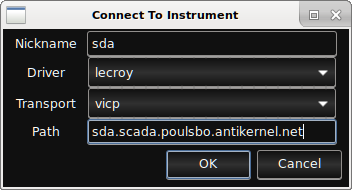
\includegraphics[width=6cm]{images/connection-dialog.png}
\caption{Connection dialog}
\label{connection-dialog}
\end{figure}

It is also possible to connect to arbitrarily many instruments by passing the ``connection string" for each instrument
as a command-line argument.

\begin{lstlisting}[language=sh]
./glscopeclient --debug \
	mylecroy:lecroy:vicp:myscope.example.com:1234 \
	myrigol:rigol:lan:rigol.example.com
\end{lstlisting}

The \texttt{--debug} argument may be omitted or replaced with any other liblogtools argument for controlling console
debug verbosity (\texttt{--quiet}, \texttt{--verbose}, \texttt{--debug}, \texttt{--trace}, etc). If you're using
glscopeclient at its current level of maturity you're probably a developer, so we suggest \texttt{--debug} by default.

Each instrument is described by a ``connection string" containing four colon-separated fields.

\begin{itemize}
\item Nickname. This can be any text string not containing spaces or colons. If you have only one instrument it's
largely ignored, but when multiple instruments are present channel names in the UI are prefixed with the nickname to
avoid ambiguity.
\item Driver name. This is a string identifying the command protocol the scope uses. Note that not all
scopes from the same vendor will use the same command set or driver!
\item Transport. This is is a string describing how the driver connects to the scope (e.g. RS232 or Ethernet)
\item Arguments for the driver identifying the device to connect to, separated by colons. This varies by driver but is
typically a hostname:port combination, TTY device path, or similar.
\end{itemize}

\section{Design Philosophy}

glscopeclient's UI is heavily mouse driven and context based. Space used by always-visible buttons, sliders, etc is
kept to a minimum in order to keep as much screen real estate as possible usable for waveform display. Additional
controls are displayed in menus or pop-up dialogs, then hidden as soon as they are not needed.

Most UI elements can be interacted with by left clicking (select), left dragging (move), using the scroll wheel (zoom),
double clicking (open properties dialog), or right clicking (context menu).

Most text fields allow SI prefixes for scaling values (mV, us, GHz, etc).

\section{Troubleshooting}

\subsection{Corrupted or no graphical output in waveform areas}

Some users have reported problems with libglvnd under Linux. Changing the CMP0072 declaration in
glscopeclient/CMakeLists.txt from NEW to OLD may fix it.
